\documentclass{beamer}
%\documentclass[handout]{beamer}

\mode<presentation>
{% AnnArbor
%\usetheme{AnnArbor}
  %\usetheme{Boadilla}
  \usetheme{CambridgeUS}
 %\usetheme{Madrid}
  \setbeamercovered{transparent}
}

\usepackage{fontspec,xltxtra,xunicode,moreverb}

\usepackage[french]{babel}
% \usepackage{beamerthemesplit} // Activate for custom appearance

%% No navigation symbol.
\setbeamertemplate{navigation symbols}{}
\beamertemplatenavigationsymbolsempty

%\setbeameroption{hide notes}
\newcommand{\mypause}{\pause}
% \newcommand{\mypause}{~}

\newcommand{\elvrm}{\rm}
\newcommand{\fivrm}{\rm}
\newcommand{\sixrm}{\rm}
\newcommand{\sevrm}{\rm}
\newcommand{\egtrm}{\rm}
\newcommand{\ninrm}{\rm}
\newcommand{\tenrm}{\rm}
\newcommand{\twlrm}{\rm}
\newcommand{\frtnrm}{\rm}
\newcommand{\svtnrm}{\rm}
\newcommand{\twtyrm}{\rm}
\newcommand{\twfvrm}{\rm}

\newcommand{\ex}{{\bf Exemple}}
\newcommand{\afor}{\bf for}
\newcommand{\ato}{\bf to}
\newcommand{\ado}{\bf do}
\newcommand{\aendo}{\bf endo}
\newcommand{\esp}{\hspace{0.5cm}}

\newcommand{\sal}{\sum_i \mu_i}
\newcommand{\sbet}{\sum_j \nu_j}
\newcommand{\If}{\mbox{\bf if }}
\newcommand{\Then}{\,\mbox{\bf then }}
\newcommand{\titre}[1]{\title{{{\color{red} \large \bf #1}}}}

% Needed for course 2.
\newcommand{\Zn}{{\bf Z}^n}
\newcommand{\Z}{{\bf Z}}
\newcommand{\N}{{\bf N}}
\newcommand{\Np}{{\bf N}^p}

\newcommand{\alfa}{\textsc{alpha}}
\newcommand{\alfacase}{\mbox{\bf case}}
\newcommand{\alfaesac}{\mbox{\bf esac}}
\newcommand{\zset}{\mathbb{Z}}

\newcommand{\sys}{{\bf system}}
\newcommand{\real}{{\bf real}}
\newcommand{\of}{{\bf of}}
\newcommand{\lett}{{\bf let}}
\newcommand{\tel}{{\bf tel}}
\newcommand{\returns}{{\bf returns}}
\newcommand{\boolean}{{\bf boolean}}
\newcommand{\true}{{\bf true}}
\newcommand{\false}{{\bf false}}

\newcommand{\pomme}{\texttt{cmd}}
\newcommand{\alalign}{{$\hookleftarrow$}}

\newcommand{\pyth}{{\sc Python}}
\newcommand{\prog}[1]{\alert{\texttt{#1}}}

\title{Introduction à l'informatique}
% \author{Patrice Quinton}
\author{Lilian Besson}
\date{2018\\Version du \today}

\institute% (optional, but mostly needed)
{ENS Rennes}

\date%[\today] % (optional, should be abbreviation of conference name)
[Info - DEM - 2020]{Initiation à l'informatique -- DEM -- 2020\\Module 2}%\logo{
\includegraphics[height=0.5cm]{logoENS.pdf}}

\pgfdeclareimage[height=0.5cm]{adb-logo}{logoENS.pdf}
\logo{\pgfuseimage{adb-logo}}

% Delete this, if you do not want the table of contents to pop up at
% the beginning of each subsection:
\AtBeginSection[]
{
  \begin{frame}<beamer>
    \frametitle{Plan du cours}
%    \tableofcontents[currentsection,currentsubsection]
\tableofcontents[currentsection,currentsubsection,hideallsubsections]
  \end{frame}
}

\begin{document}

\frame{\titlepage}

\section[Outline]{}
\frame{\tableofcontents}

\frame
{
\frametitle{\emph{``Résumé de l'épisode précédent''}}
{
  \begin{itemize}
  \item \prog{Algorithme} = procédé systématique pour résoudre un problème \mypause{}
  \item \prog{Algorithme} $\not = $ \prog{Programme}\mypause{}
  \item \prog{Ordinateur} = machine à interpréter du texte\mypause{}
  \item On s'adresse à un ordinateur d'abord via un \prog{terminal} qui permet
un dialogue à base de commandes\mypause{}
  \item L'interface graphique est une \prog{métaphore} bien pratique pour
accéder à des applications
  \end{itemize}
}
}

\section{\pyth{}, un langage, pour communiquer avec l'ordinateur}

\frame
{
\frametitle{Démarrer Python}
{\footnotesize
\begin{itemize}
\item Double-cliquez sur l'icône de \prog{idle} dans le menu de vos applications (peut être dans un sous dossier nommé Python), ou tapez la commande \prog{idle \&} dans un terminal.\mypause{}
\item Vous devez voir s'ouvrir une nouvelle fenêtre. Cette fenêtre vous donne accès à l'interpréteur
du langage \pyth{} \mypause{}
\item Tapez la commande \texttt{\prog{2+2}} dans cette fenêtre puis \alalign{}\mypause{}
\item Ouvrez une fenêtre de l'éditeur \prog{idle} (\prog{New} dans le menu \prog{File})\mypause{}
\item Tapez une petite expression, par exemple \prog{print(2+2)} dans cette fenêtre \prog{File} \mypause{}
\item Puis, sauvegardez ce petit texte dans un programme appelé \prog{essai1.py}. Pour ce faire\mypause{}
\begin{itemize}
\item Choisissez la commande \prog{Save as} dans le menu déroulant \prog{File}
\item Une fenêtre vous demandera sous quel nom sauvegarder votre fichier\mypause{}
\end{itemize}\mypause{}
\item Maintenant, exécutez votre programme avec la commande \prog{Run Module (F5)} du menu
\prog{Run}\mypause{}
\item Si tout s'est bien passé, l'interpréteur \pyth{} vous a donné la réponse dans l'autre fenêtre
\end{itemize}
}
}


\frame
{
\frametitle{Que s'est-il passé?}
{\footnotesize
\begin{itemize}
\item La commande \prog{idle \&} vous a permis d'accéder à un \alert{{\em l'interpréteur}}
de programmes \pyth{}. \mypause{}
\item Avec la commande \prog{New}, on a ouvert une nouvelle fenêtre permettant
l'accès à \prog{l'éditeur} de \pyth{}\mypause{}
\item Cet éditeur est utilisable \alert{en parallèle} avec votre terminal (à cause du petit caractère
\prog{\&} à la fin): vous pouvez utiliser l'un ou l'autre, en déplaçant votre souris. On appelle chacun
de ces programmes des \alert{processus}\mypause{}
\item Cet éditeur vous a permis de taper un petit programme \pyth{}, de le sauvegarder
dans votre répertoire courant. Allez dans votre fenêtre de commande, et vérifiez
avec la commande \prog{ls} qu'il y est bien.\mypause{}
\item La commande \prog{Run Module (F5)} a lançé un troisième processus, permettant
d'accéder à l'interpréteur \pyth{}. Elle a aussi demandé à ce processus qu'il lise et exécute
le programme qui est contenu dans la fenêtre de l'éditeur \prog{idle}. \mypause{}
\item Vous pouvez passer d'une \alert{fenêtre} à l'autre \\
  (ou ce qui revient au même, d'un \alert{processus} à l'autre).
\end{itemize}
}
}

\frame
{
\frametitle{Remarque}
\begin{itemize}
\item Lorsqu'on lance \pyth{} par double-click, on ne sait pas où il sauve les fichiers...\mypause{}
\mypause{}
\item À un instant donné, \pyth{} est toujours "lié" à un répertoire particulier\mypause{}
\item Pour le connaître, taper \prog{import os} et \prog{os.getcwd()}
dans la fenêtre interpréteur: la commande \prog{import} charge
un module contenant plein de fonctions liées au système d'exploitation (os),
dont celle qui permet d'obtenir le répertoire courant (\prog{getcwd})
\end{itemize}
}

\frame
{
\frametitle{L'interpréteur \pyth{}}
\begin{itemize}
\item \pyth{} est un \textbf{programme} de votre ordinateur (comme une \emph{appli} sur votre téléphone)\mypause{}
\item C'est un \alert{interpréteur}:
  \begin{itemize}
    \item
    il lit un programme,
    \item
    ligne par ligne,
    \item
    et exécute ce programme au fur et à mesure de son interprétation
  \end{itemize}
  \mypause{}
\item D'autres langages sont \alert{compilés} (comme \texttt{C} ou \texttt{JAVA} ou \texttt{OCaml} par exemple): le \alert{compilateur} les lit, et les traduit dans une autre format, lisible directement par l'ordinateur (langage \emph{binaire}), plus efficace.
\end{itemize}
}


\frame
{
\frametitle{La fenêtre \pyth{}}
\begin{itemize}
\item On accède à l'interprète de \pyth{} de façon directe, par la fenêtre \pyth{}  \mypause{}
\item Cette fenêtre donne accès à {\em l'environnement} d'exécution de
\pyth{}  \mypause{}
\item À chaque fois qu'on exécute une {\em commande} (aussi appelée, une
\alert{instruction}), on modifie \alert{l'environnement} de \pyth{}  \mypause{}
\end{itemize}

\begin{block}{Exemple}
\begin{itemize}
\item On tape \prog{10+20} dans la fenêtre, puis \alalign{}
\item Résultat: \prog{30}
\end{itemize}
\end{block}
}

\frame
{
\frametitle{La fenêtre \pyth{}}
\begin{block}{Que s'est-il passé?}
\begin{itemize}
\item \pyth{} a interpreté une \alert{\em expression} et
affiché sa valeur \mypause{}
\item La fenêtre \pyth{} présente sous forme lisible le comportement
de l'interpréteur \pyth{}, qui réalise indéfiniment le boucle suivante:
  \begin{itemize}
  \item lire une séquence de caractères (ici, \prog{10 + 20}) fournie par
  l'utilisateur.
  \item l'interpréter, et réaliser les opérations correspondant
  à cette interprétation: additionner \prog{10} et \prog{20}, puis afficher
  le résultat, et enfin, imprimer un prompt (\prog{>>> }).
  \end{itemize}
\end{itemize}
\end{block}
}

\section{Premiers programmes}

\frame
{
\frametitle{\'Evaluer des expressions entières}
\begin{block}{Par des exemples}
{\footnotesize
\begin{itemize}
\item \prog{10} est un entier (un \prog{int})  \mypause{}
\item \prog{-10} aussi. Si une expression \prog{e} est un entier, alors \prog{+e} ou \prog{-e} le sont aussi  \mypause{}
\item \prog{10 + 20} est aussi un entier. D'ailleurs, si \prog{e} et \prog{f} sont des entiers,
alors \prog{e + f}, mais aussi \prog{e - f} ou \prog{e * f} sont des expressions entières  \mypause{}
\item Mais aussi \prog{e // f} qui donne le résultat de la \alert{division entière} de \prog{e} par
\prog{f}  \mypause{}
\item Mais aussi \prog{e \% f} qui donne \prog{le reste} de la \alert{division entière} de \prog{e} par
\prog{f}  \mypause{}
\item On peut parenthéser les expressions: si \prog{e} est une expression entière, alors
\prog{(e)} l'est aussi
\end{itemize}
\end{block}
}
}

\frame
{
\frametitle{Exercice M2.1}
\begin{block}{Faire}
  {\footnotesize
Pour évaluer une expression \prog{e}, on tape cette expression (dans la fenêtre \pyth{}), et on va à la ligne
\begin{itemize}
\item Evaluez \prog{10 + 20}, puis \prog{-20}, puis \prog{4*2}, puis \prog{5 // 2}, et enfin \prog{5 \% 2} \mypause{}
\item Dites-moi ce que vous observez?  \mypause{}
\end{itemize}
\end{block}

\begin{block}{Observer}
\begin{itemize}
\item Vous devez trouver les valeurs prévues: \prog{30}, \prog{-20}, \prog{8}, \prog{2}
et \prog{1}
\end{itemize}
\end{block}
}
}

\frame
{
\frametitle{Exercice M2.2}
\begin{block}{Faire}
  {\footnotesize
On peut mémoriser plusieurs expressions à calculer dans un fichier, et exécuter le contenu
de ce fichier. Mais, rien ne se passe, si l'on ne demande pas au programme d'imprimer
le résultat, ce qui se fait avec la fonction \prog{print(expression)}.
\begin{itemize}
\item Tapes les formules \prog{print(10 + 20)}, puis \prog{print(-20)}, etc, dans une fenêtre que vous ouvrez et
que vous sauvegardez avant de l'exécuter. \mypause{}
\item Ajoutez-y \prog{print("Le résultat de 10 + 20 est :", 10+20)}.
\item Dites-moi ce que vous observez?  \mypause{}
\end{itemize}
\end{block}

\begin{block}{Observation}
\begin{itemize}
\item Vous devez voir s'afficher les valeurs prévues: \prog{30}, \prog{-20}, \prog{8}, \prog{2}
et \prog{1}  \mypause{}
\item Elles sont affichées ligne par ligne (une par \prog{print})
\end{itemize}
\end{block}
}
}

\frame
{
\frametitle{Exercice M2.3}
\begin{block}{Faire}
  {\footnotesize
\prog{10}, \prog{-2} etc. sont des \prog{entiers} (en \pyth{} des \prog{int}).
Par contre, \prog{10.0} ou \prog{-10.2} sont des \prog{réels} (ou flottants).
\begin{itemize}
\item Tapes les formules \prog{print(10.0 + 20.0)}, puis \prog{print(-20.0)}, etc, dans une fenêtre que vous ouvrez et
que vous sauvegardez avant de l'exécuter. \mypause{}
\item Ajoutez-y \prog{print( "Le résultat de 10.0 + 20.0 est :", 10.0 + 20.0)}.
\item Que donne le calcul \prog{print(10.0 + 20)}?
\item Dites-moi ce que vous observez?  \mypause{}
\end{itemize}
\end{block}

\begin{block}{Observation}
\begin{itemize}
\item Vous devez voir s'afficher les valeurs prévues: \prog{30.0}, \prog{-20.0}, \prog{8}, \prog{2}
et \prog{1}  \mypause{}
\item Le calcul \prog{10.0 + 20} donne un résultat flottant : il y a une {\em conversion}.
\end{itemize}
\end{block}
}
}


\frame
{
\frametitle{Variables, mémoire}
% {\footnotesize
\begin{itemize}
\item Tout ordinateur est doté d'une mémoire\mypause{}
\item Un programme est un moyen d'effectuer des calculs, de les mémoriser.\mypause{}
\item \pyth{} accède à sa mémoire via des {\em variables}: des noms qui font référence
à des valeurs mémorisées. \mypause{}
\item Si on donne à évaluer \prog{x = 10} (dans le fenêtre \pyth{}), il ne se passe
rien de visible, mais \pyth{} associe à \prog{x} la valeur entière \prog{10}.\mypause{}
\item On le voit si on évalue \prog{x}.
\item En tapant \prog{type(x)}, on voit que \pyth{} a choisi de donner à \prog{x} le type
\prog{int}.
\end{itemize}
% }
}

\frame
{
\frametitle{Exercice M2.4}
{\footnotesize
\begin{block}{Faire}
\'Ecrire et exécuter un petit programme qui:
\begin{itemize}
\item Met dans une variable \prog{x} la valeur \prog{10},
\item dans une variable \prog{y} la valeur \prog{20},
\item et dans une troisième variable \prog{z} la somme de \prog{x + y} et affiche cette
valeur.
\end{itemize}
\end{block}

\begin{block}{Solution (?)}
\prog{
\begin{tabular}{l}
x = 10\\
y = 20\\
\texttt{print("La somme de x et y est :", z)}
\end{tabular}
}
\end{block}

}
}



\frame
{
\frametitle{Commentaires}
{
Tout ce qui suit le caractère \prog{\#} est un commentaire, ignoré par \pyth{}.\\
Mais utile pour :
\begin{itemize}
  \item vous : quand vous relisez votre code,
  \item vos camarades, vos collègues.
\end{itemize}

\begin{block}{~}
Exemple:

\prog{
\begin{tabular}{l}
\texttt{\# On définit x et on lui donne la valeur 10}\\
x = 10\\
\texttt{\# On définit y et on lui donne la valeur 20}\\
y = 20\\
\texttt{\# On additionne x et y, résultat dans z}\\
z = x + y\\
\texttt{print("La somme de x et y est :", z)}
\end{tabular}
}
\end{block}
}
}



\section{Conclusion}
\frame
{
\frametitle{En résumé}
\begin{itemize}
\item Vous avez pris connaissance de votre système d'exploitation (\alert{Linux},
\prog{Mac OS}, \prog{Windows})\mypause{}
\item Vous avez eu un premier contact avec \alert{\pyth{}} et son éditeur \alert{\texttt{idle}}\mypause{}
\item Vous avez appris à évaluer quelques \alert{expressions simples}\mypause{}
\item Vous avez écrit vos premiers programmes, pour des calculs arithmétiques\mypause{}
\item Premier contact avec la notion de variable (\prog{x}, \prog{y}, \prog{z} dans les exemples précédents)

\item[$\rightarrow$:] Module 3: on continue \pyth{} !
\end{itemize}
}



\section{Petite histoire : compilation vs interprétation, et Grace Hopper}
\frame
{
\frametitle{Langages compilés vs interprétés}
\begin{itemize}
  \item Comme nous l'avons vu, \prog{python} est un \alert{programme} qui lit et \alert{interprète} des commandes ou des fichiers écrits en \pyth{} \mypause{}
  \item Il existe des milliers de langages de programmation, les deux grandes familles étant \mypause{}
  \begin{itemize}
    \item les \textbf{langages interprétés}, comme Python ou les langages de shell utilisés par le terminal (\prog{bash}, \prog{sh}, PowerShell sur Windows) \mypause{}\\
      Ex: \prog{fichier.py} $\rightarrow$ lu par \prog{python} $\rightarrow$ \emph{interprété} par \prog{python} \mypause{}
    \item les \textbf{langages compilés}, les deux plus populaires étant \prog{C} et \prog{JAVA} (utilisé pour les applis Android), ou encore \prog{Swift} pour les applis iOS (Apple) \mypause{}\\
      Ex: \prog{fichier.c} $\rightarrow$ lu par \prog{gcc} $\rightarrow$ \prog{fichier.s} assembleur $\rightarrow$ lu par \prog{gcc} $\rightarrow$ \prog{fichier.exe} binaire $\rightarrow$ \emph{exécuté directement par le processeur} \mypause{}
      \item il y a des intermédiaires, par exemple utilisant des machines virtuelles (eg JVM pour JAVA) mais cela va au delà du contenu du cours.
    \end{itemize}
\end{itemize}
}

\frame
{
\frametitle{Pause ``culture geek'' : code assembleur dans Terminator}
{
  \footnotesize
  Dans le film Terminator (1984) de James Cameron, un robot venu du futur (le Terminator T800) poursuit une jeune femme (Sarah Connor).\\
  Quelques passages montrent ce que voit le robot, et pour ``faire encore plus informatique'', du code assembleur est affiché sur le côté :

  \begin{figure}
    \center
    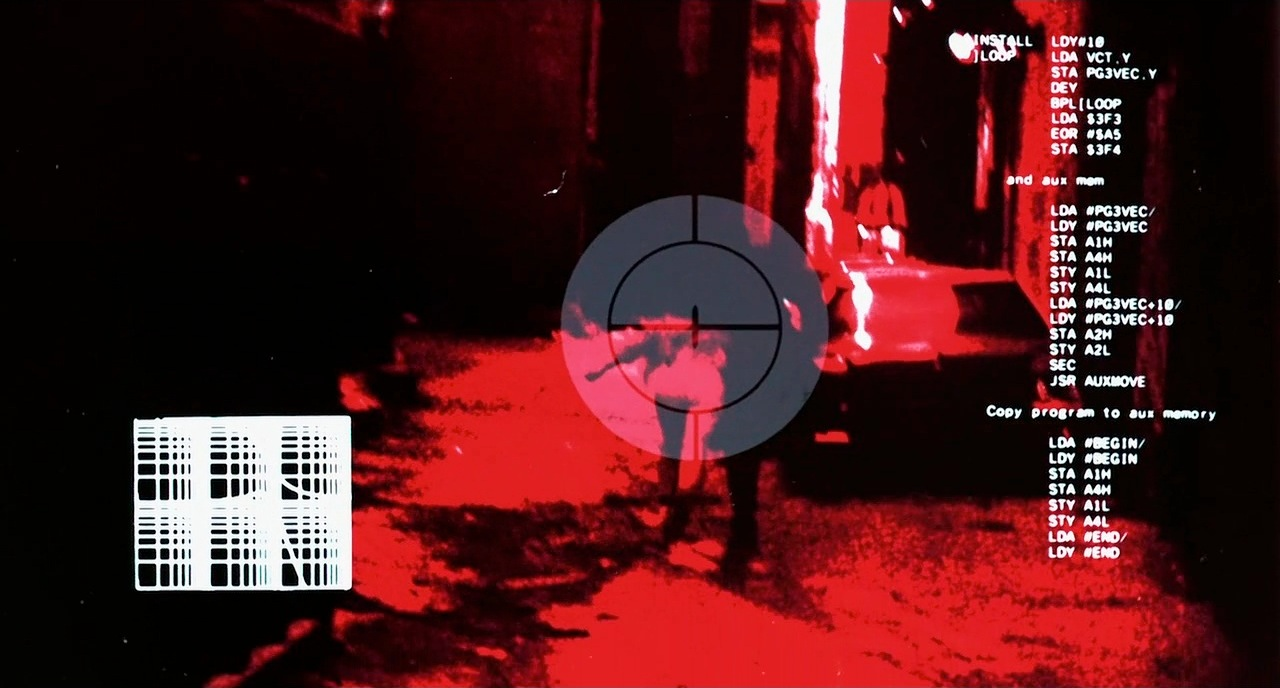
\includegraphics[height=125pt]{00-37-19.jpg}
  \end{figure}
  (source et explications sur \prog{https://www.pagetable.com/?p=64})
}
}

\frame
{
\frametitle{Grace Hopper : inventrice du premier compilateur}
  \vspace*{125pt}
  \begin{figure}
    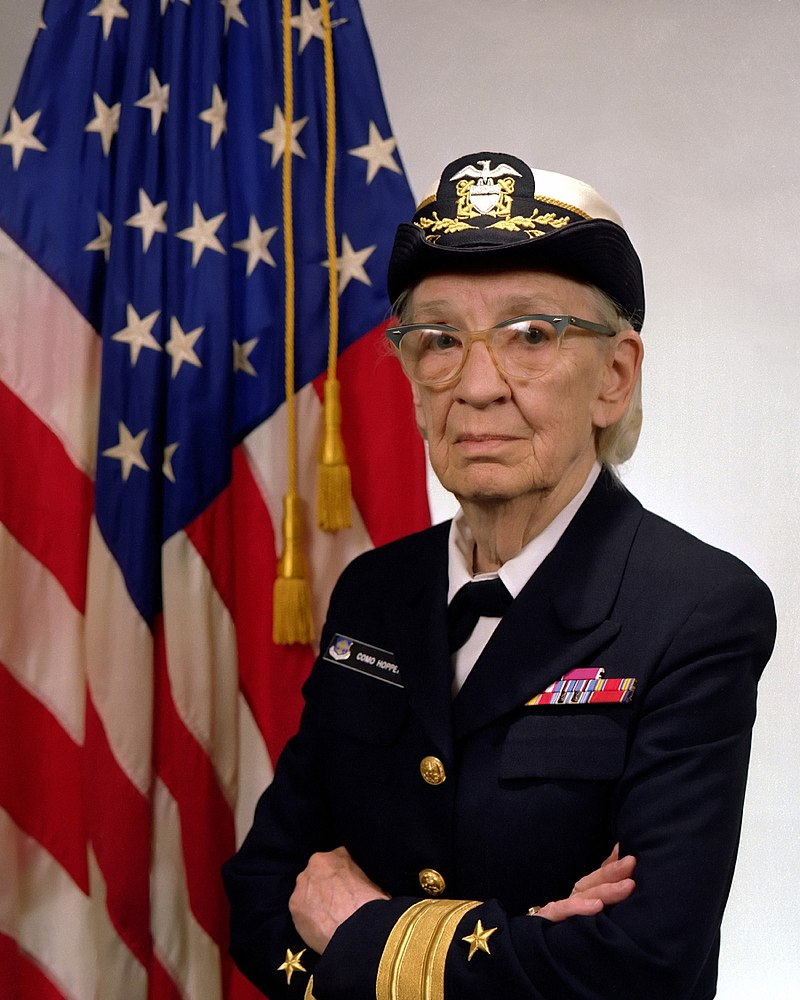
\includegraphics[height=10pt]{Commodore_Grace_M._Hopper_USN.jpg}
  \end{figure}
  \begin{itemize}
    \item Grace Murray Hopper, née en 1906 et morte en 1992, est une informaticienne américaine et Rear admiral de la marine américaine
  \end{itemize}
}

\frame
{
\frametitle{Grace Hopper : inventrice du premier compilateur}
\begin{itemize}
\item Engagée dans l'armée des USA en 1943, elle travaille au \emph{Bureau of Ordnance Computation Project} de l'université Harvard et fait partie des premières personnes à apprendre à programmer le premier ordinateur éléctromécanique, le IBM ASCC (Harvard Mark-1) \mypause{}
\item Elle est la conceptrice du premier compilateur en 1951 (A-O system)
\item et contribue à la création du langage \prog{FORTRAN} en 1954 (encore utilisé aujourd'hui) et \prog{COBOL} en 1959 \mypause{}
\item On lui devrait le nom \emph{bug} (bogue) pour le concept d'un problème survenu lors de l'exécution d'un programme en informatique...
  Selon la légende, une mite s'était logée dans un trou d'une carte perforée, découverte par Grace Hopper en constatant une erreur de calcul de cette machine à cartes perforées.
\end{itemize}
}



\end{document}
